\documentclass[a4paper]{article}

%% Language and font encodings
\usepackage[spanish]{babel}
\usepackage[utf8x]{inputenc}
\usepackage[T1]{fontenc}
\usepackage{listings}
\spanishdecimal{.}


%% Sets page size and margins
\usepackage[a4paper,top=3cm,bottom=2cm,left=3cm,right=3cm,marginparwidth=1.75cm]{geometry}

%% Useful packages
\usepackage{amsmath}
\usepackage{graphicx}
\usepackage[colorinlistoftodos]{todonotes}
\usepackage[colorlinks=true, allcolors=blue]{hyperref}

\title{Práctica 10: algoritmo genético}
\begin{document}
\maketitle

\section{Introducci\'on}
En esta tarea se aborda uno de los problemas más populares y trabajados en la rama de la optimización, se trata de el problema de la mochila, el cual consiste en decidir que objetos colocas o seleccionas para llevar en una mochila, considerando que tiene cierta capacidad de objetos y cuyo objetivo es obtener el máximo beneficio. La tarea diez consiste en paralelizar el código dado, el cual se resuelve por medio de un algorítmo genético, y argumentar estadísticamente que la paralelización entrega una solución en menor tiempo que de la forma secuencial.

\section{Par\'ametros de trabajo}
La experiemtnación se realizó en un HP Z230 Tower Workstation con procesador Intel(R) Xenon(R) CPU E3-1240 v3 y 3.40 GHz de memoria ram 16 GB y un sistema operativo de 64 bits con Windows 7 Home Premium.

La población inicial a lo largo de la práctica varía entre $n\in\{20,50,100,200,350,400\}$, seleccionando estos valores tras un diseño de experimentos siendo los más convenientes en tiempos, como para esta parte solo nos interesa comparar los tiempos y es de suponerse que el tiempo que tarda en realizar una generación es similar independientemente de el número de generaciones que realice, para esta primer fase fue seleccionado un número pequeño $g=5$.


\section{Modificaciones del código}
Se agregaron los comandos necesarios para la paralelización, para efecto práctico se mostrará el modo de paralelizar solo una de las funciones, la función \texttt{mutar}, de forma similar se realizó para el resto de las mismas, tomando en cuenta que no toda función que se establece en el código base se paralelizó ya que algunas por su modo de estructura es simplemente imposible paralelizarlas. 

\begin{lstlisting}[frame=single]
library(parallel)
cluster <- makeCluster(detectCores() - 1)
  clusterExport(cluster, "pm")
  clusterExport(cluster, "p")
  clusterExport(cluster, "mutacion")
  clusterExport(cluster, "n")
  clusterExport(cluster, "tam")
  clusterExport(cluster, "fun.mutar")
  ...
  vec.mutados <- parSapply(cluster, 1:tam, fun.mutar)
  vec.mutados <- unlist(vec.mutados)
  ...
  stopCluster(cluster)
\end{lstlisting}

Así mismo se incluyeron los comandos de medición de tiempo y los ciclos \texttt{for} necesarios para la automatización del cambio de población inicial. Los resultados de los tiempos se guardan en un archivo tipo \texttt{csv}, los cuales en un inicio están almacenados en una variable tipo \texttt{data.frame}, esto con el fin de ir salvando los tiempos por ciclo de población inicial.
\begin{lstlisting}[frame=single]
tiemposec <- data.frame()
...
valss<-c(20,50,100,200,350,400)
for(i in 1:(length(valss))){
init <- valss[i]
...
tmax <- 5
....
for (iter in 1:tmax) {
c <- Sys.time()
...
 d <- Sys.time()
 ti <- c(c,d)
 tie <- diff(ti,units="secs")
 tiemposec <- rbind(tiemposec,c(init,tie))
 } }
 ...
 write.csv(tiemposec, file="TiemposP.csv")
\end{lstlisting}

\section{Resultados y conclusiones}
En la figura \ref{fig:ambos} podemos observar de forma clara la diferencia de tiempos de ejecución. Las instrucciones de la práctica especifican que se requiere una prueba estadística para la justificación de la paralelización, pero al notar la gran diferencia de tiempos se cree innecesario realizarla, es por esto que se cambiaron los tamaños de la población con el fin de observar si al ser una muestra más pequeña de población en algún punto era mejor la forma secuencial del código, pero ni de esta manera los tiempos llegan a aproximarse, es sin duda la forma paralelizada la que requiere menos de una tercera parte del tiempo que toma en forma secuencial.

\begin{figure}[h!]
\centering
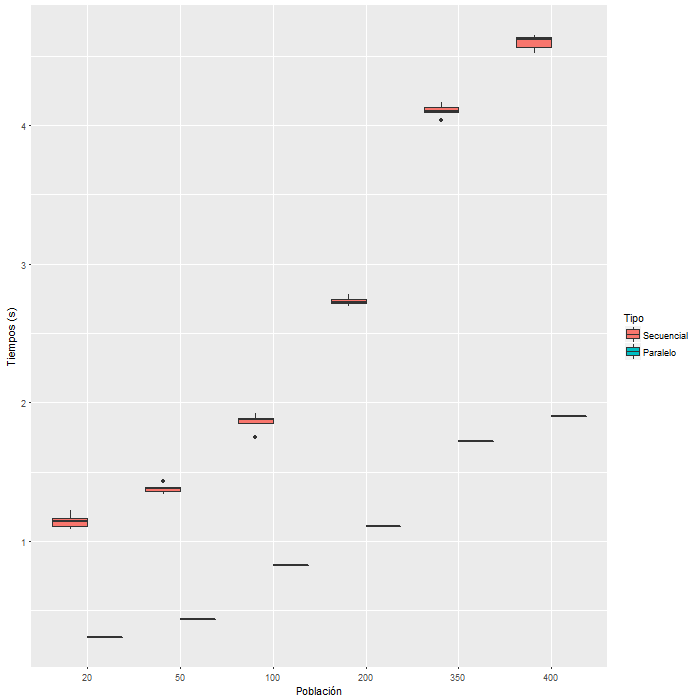
\includegraphics[width=0.7\linewidth]{ambos}
\caption{Tiempos de ejecución por tamaño de población para el código secuencial, así como para el paralelizado.}
\label{fig:ambos}
\end{figure}


\section{Reto 1}
El primer reto consiste en modificar la función de selección de padres de tal forma que el algoritmo tome los padres en base a una probabilidad establecida en proporción con su aportación al valor objetivo. En este caso la finalidad no es ver el cambio en los tiempos de ejecución sino la mejora en la solución final, es decir en mi diferencia con el óptimo del problema. Para esto solo fue necesario hacer uso del parámetro \texttt{prob} en la función \texttt{sample}.

\section{Modificación del código y parámetros de R1}
Para este reto fue necesario realizar algunos cambios al código paralelizado, se retiraron los comandos de medición de tiempo, se mantuvo el ciclo de variación de población pero con una ligera modificación, siendo los valores utilizados $n\in\{20,50,70,100\}$,se incluyó un ciclo \texttt{for} con el fin de reproducir para cada una de las poblaciones la experimentación diez veces. De igual forma que al salvar los tiempos, fue necesario crear un \texttt{dat.frame}, este con el fin de guardar los valores de la solución como la diferencia con el óptimo para cad réplica. El cantidad de las generaciones en esta ocación aumento, ya que al buscar la mejora de la solución era indispensable aumentar el valor, se estableció $g=70$.
\begin{lstlisting}[frame=single]
valobj <- data.frame()
valss<-c(20,50,70,100)
for(va in 1:4){
for(la in 1:10){
init <- valss[va]
tmax <- 70
  valobj<-rbind(valobj,c(init,mejor, (optimo - mejor) / optimo))
  }}
\end{lstlisting}
Por otra parte para la modificación de la función lo necesario fue calcular la probabilidad a asignar, es decir saber cuanto aporte daba cada una de las soluciones y pasar estos datos al momento de paralelizar la función.
\begin{lstlisting}[frame=single]
      s <- c()
      s <- parSapply(cluster, 1:tam, val.objetivo)
      su <- sum(s)
      pobj <- rep(0,tam)
      
      for(a in 1:init){
      pobj[a] <- (s[a]/su)
      }
      ...
fun.reproduccion <- function(i){
	padres <- sample(1:tam, 2, replace=FALSE,prob = pobj)
	hijos <- reproduccion(p[padres[1],], p[padres[2],], n)
	return(hijos)
}
\end{lstlisting}
\section{Resultados y conclusiones de R1}
Con el fin de observar si la mejora de las soluciones era más rápida con la asignación de probabilidad se ilustra en la figura \ref{fig:tendencia} el comportamiento del \texttt{GAP}, es decir la diferencia con respecto al óptimo.
\begin{figure}[h!]
\centering
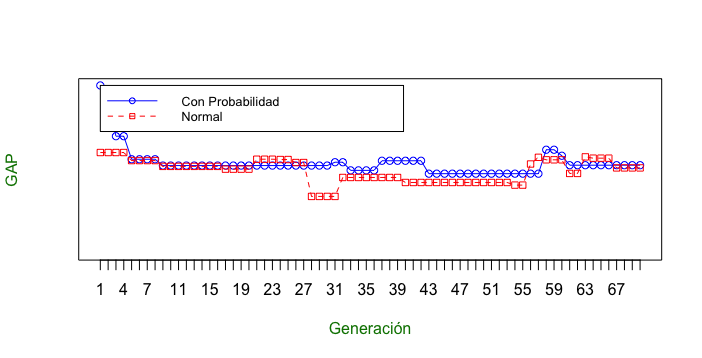
\includegraphics[width=0.7\linewidth]{tendencia}
\caption{Tendencia del GAP respecto al avance de generaciones.}
\label{fig:tendencia}
\end{figure}

Des afortunadamente de lo anterior no se puede argumentar mucho, ya que aunque la linea que nos representa el modo de elección de los padres de manera normal pareciera estar en gran medida estar bajando, en gran parte de las generaciones existe un traslape de las lineas.

\begin{figure}[h!]
\centering
\includegraphics[width=0.7\linewidth]{Reto1}
\caption{Desviación con el óptimo de diez repeticiones respecto al cambio de población.}
\label{fig:Reto1}
\end{figure}

Con la figura \ref{fig:Reto1} es algo notorio cual de las dos formas de selección de padres es más conveniente para acercarse al óptimo, pero de igual forma es necesaria alguna prueba estadística que lo sustente. A simple vista el que tiene una desviación menor en los cuatro tamaños de población es cuando la probabilidad es asignada. La primera prueba que es necesaria sirve para saber si mis datos son normales, para saber que clase de prueba es necesaria aplicar, en nuestro caso una prueba de \texttt{Shapiro} nos indica que los valores no son normales, por tanto es necesario realizar una prueba no para-métrica.
\begin{lstlisting}[frame=single]
Shapiro-Wilk normality test

data:  ambos$Diferencia
W = 0.9887, p-value = 0.7114
\end{lstlisting}

Se lleva a cabo una prueba \texttt{Wilcoxon} con el fin de saber si hay una diferencia significativa en las medias.
\begin{lstlisting}[frame=single]
Wilcoxon rank sum test
data:  ambos$Diferencia[ambos$Tipo == "Probabilidad"] and 
ambos$Diferencia[ambos$Tipo == "Normal"]
W = 383, p-value = 3.795e-05
alternative hypothesis: true location shift is not equal to 0
\end{lstlisting}
Nuestro indicador es el  $p$-value, el cual nos confirma que existe una diferencia significativa en las medias, es por esto que se procede a medir que tanta diferencia hay y cual de ellas es menor.

\begin{lstlisting}[frame=single]
> median(ambos$Diferencia[ambos$Tipo=="Probabilidad"])
[1] 0.09074176
> median(ambos$Diferencia[ambos$Tipo=="Normal"])
[1] 0.1116319
\end{lstlisting}

De la anterior prueba podemos argumentar que efectivamente existe una menor desviación del óptimo al asignar las probabilidades que al dejar que la selección se lleve a cabo de forma normal.

\section{Reto 2}
Para el reto dos lo que se espera analizar es similar al reto uno, solo que en este caso en lugar de modificar la probabilidad de selección de padres se modificará la supervivencia de las mejores soluciones.

\section{Modificación de código y parámetros R2}
Los parámetros se mantienen igual que en el reto 1, es decir la misma cantidad de generaciones y la misma variabilidad respecto a población. Para las modificaciones del código fue necesario verificar que los valores al momento de evaluar en la función existieran y reasignar las probabilidades respecto al valor objetivo, de igual forma que se realizó en el reto uno para esto se creó un nuevo vector.

\begin{lstlisting}[frame=single]
probabilidad <- c()
pro<-c()
for(indi in 1:tam){
if(is.na(p$fact[indi])){
p$obj[indi]=0
}}
suma <- sum(p$obj)
for(indi in 1:tam){
pro <- (p$obj[indi])/suma
probabilidad <- c(probabilidad,pro)
}
p$probabilidad <- c(probabilidad)
...
mantener <- sample(1:tam, init, replace=FALSE, prob = p$probabilidad)
\end{lstlisting}

\section{Resultados y conclusiones de R2}
\begin{figure}[h!]
\centering
\includegraphics[width=0.7\linewidth]{Reto2}
\caption{GAP respecto a la cantidad de población, cada una con diez iteraciones.}
\label{fig:Reto2}
\end{figure}

De igual forma que en el reto uno podemos visualizar con la figura \ref{fig:Reto2} que en cuanto a mejora de soluciones es mejor utilizar la manera normal, es decir sin asignar probabilidades según la mejor.En este caso la prueba de normalidad \texttt{Shapiro} nos indica que los valores no son normales. Se lleva a cabo una prueba \texttt{Wilcoxon} con el fin de saber si hay una diferencia significativa en las medias.
\begin{lstlisting}[frame=single]
	Wilcoxon rank sum test
	data:  ambos$Diferencia[ambos$Tipo == "Pro"] and ambos$Diferencia[ambos$Tipo == "Normal"]
	W = 919, p-value < 2.2e-16
\end{lstlisting}
El  $p$-value, el cual nos confirma que existe una diferencia significativa en las medias, y de igual forma se midió que tanta diferencia hay y cual de ellas es menor.

\begin{lstlisting}[frame=single]
> median(ambos$Diferencia[ambos$Tipo=="Pro"])
[1] 0.2425497
> median(ambos$Diferencia[ambos$Tipo=="Normal"])
[1] 0.1116319
\end{lstlisting}
Comprobando que en este caso la mejor opción es no asignar las probabilidades.

\end{document}